\section{Arbeitsablauf des Schlussfolgerers}
Alle Axiome werden entsprechend dem MEMA-Prinzip abgelegt. Dabei ist für jedes Axiom genau eine Relation vorgesehen. Für gewisse Axiome werden implizite Informationen abgelegt, wie. z.B.

ObjectProperty Assertion a p n --> p type ObjectProperty

Falls ein Axiom aus komplexen Ausdrücken zusammengesetzt ist werden die Ausdrücke rekursiv abgearbeitet und einzeln behandelt. Zum herstellen der Beziehungen beim komplexen Axiomen werden Platzhalter für die Ausdrücke verwendet. Die Platzhalter die dabei erzeugt werden stammen von der OWLAPI aus der NodeID Klasse und folgen damit dem selben Schema wie auch bei anonymen Individuen.

Bsp:

(A int (Svf p B)) subC C
      nid1             C    subClass(nid1, C)
      nic2                  intOf(nid1, nid2)
 A         nid3             list(nid2, A, nid3)
            p B             svf(nid3, p, B)


Wenn Fakten in eine Relation geschrieben werden, wird von dieser ein Hinweis (Reason) an den Regelprozessor geschickt.

Dieser überprüft die Ursache und legt entsprechende Regeln an, die auf diese Veränderung ausgeführt werden können.

Die abzarbeitenden Regeln enthalten eine Referenz auf die Fakten, die hinzugekommen sind. Allgemein sind sie so implementiert, das sie nur auf diesen neuen Fakten arbeiten -  auf den sogenannten Deltas - dies ist allerdings nicht in allen Fällen möglich (cls-int1), sinnvoll (zu viele verschiedene Kombinationsmöglichkeiten) oder einfach zu komplex und damit fehleranfällig (prp-spo2). Falls zwei oder mehrmals eine Regel auf die selben neuen Fakten erzeugt wird bevor sie ausgelöst wird, werden die beiden Regeln zu einer zusammengefasst und können je nach Einstellung neu priorisiert werden.
--------
Durch eine spezielles Priorisierungsverfahren wäre es evtl. möglich zielgerichtet auf die Erzeugung gewisser Fakten hinzuarbeiten.

Was sind Fakten?

Was ist eine Ontologie?

Was sind Deltas?

Was ist eine Relation?
--------
All diese Regeln sind in einer Warteschleife abgelegt, die beim laden der Ontologie gefüllt wird und beim ab arbeiten, d.h. dem realisieren, der Ontologie ausgelesen wird.

Regeln können durch das Erzeugen von neuen Fakten Hinweise für an den Regelprozessor geben der daraufhin weiter Regeln anlegt und in die Warteschlange einsortiert.

Der Vorgang des realisierens ist abgeschlossen, wenn keine Regel neue Fakten und damit neue Regeln erzeugen kann.

Der OWL2 RL Regelsatz garantiert dabei, das es immer zu einem Ende der Regelanwendung kommen wird, egal ob eine gültige oder ungültige Ontologie geladen wird.

Für das Abarbeiten und Erzeugen der Regeln ist hauptsächlich der Regelprozessor verantwortlich. Hier sind noch weitere Einstellungsmöglichkeiten, wie z.B. die parallele Verarbeitung von Regeln vorhanden.

Nachfolgend eine Übersicht über einen Ablauf des Schlussfolgerers, wenn er eine neue Ontologie lädt (Standardfall).

\begin{figure}
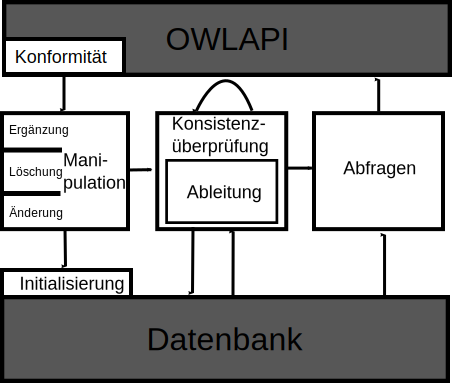
\includegraphics{images/u2r3-workflow.pdf}
\end{figure}


Speicherung

In welcher Struktur die Ontolgie in der Datenbank abgelegt wird, wurde bereits mit dem MEMA-Prinzip erklärt. Es lässt eine Speicherung zu, die sehr nach an den Axiomen aber auch den Regeln liegt und damit eine effiziente und angenehme Umsetzung der Regeln ermöglicht. Das ursprüngliche MEMA-Prinzip wurde dabei auf OWL2 angepasst und eine Möglichkeit zur Abspeicherung der Löschhierarchie erweitert. Diese ermöglicht es Schlussfolgerungen wieder gezielt rückgängig zu machen.

OWLAPI Anbindung

Der obere Teil ist die sogenannte OWLAPI. Die OWLAPI ist eine Bibliothek die das Auslesen von Ontologien in verschiedenen Formaten erlaubt und eine Schlussfolgererschnittstelle für andere Programme zur Verfügung stellt. Durch die Implementierung dieser Schnittstelle in U2R3 ist es für alle Programme zugänglich die mit der OWLAPI arbeiten.
Die Schnittstelle stellt dabei auch eine Liste typischer Abfragen für einen Reasoner dar und kann allein dadurch schon als Messlatte für die Fähigkeiten eines Schlussfolgerers verwendet werden. Das OWLAPI-Projekt ist open-source und in Java implementiert und ist damit auch optimal für die Implementierung von U2R3 geeignet. Neben der reinen Parsertätigkeit kann die OWLAPI auch noch helfen zu überprüfen, ob eine Ontologie im OWL2 RL Profil liegt und nimmt damit weitere Arbeit ab.

